\documentclass[11pt, a4paper, twocolumn]{article}

%%%%%%%%%%%%%%%%%
% Configuration %
%%%%%%%%%%%%%%%%%
\usepackage{allrunes}
\usepackage{amsmath}
% If magyar is wanted
%\usepackage[magyar]{babel}

\usepackage[T1]{fontenc}
\usepackage[utf8]{inputenc}
\usepackage{fixltx2e}
\usepackage{multirow}
\usepackage{url}
\usepackage{amsfonts}
\usepackage{amsthm}
\usepackage{amssymb}
\usepackage{xcolor}

\newcommand{\abstractText}{\noindent
  Abstract goes here.
}

% Here you can configure the layout
\usepackage{geometry}
\geometry{top=1cm, bottom=1cm, left=1.25cm,right=1.25cm, includehead, includefoot}
\setlength{\columnsep}{7mm} % Column separation width

\usepackage{graphicx}

%\usepackage{gensymb}
\usepackage{float}

% For bra-ket notation
\usepackage{braket}

% To have a good appendix
\usepackage[toc,page]{appendix}

\usepackage{abstract}
\renewcommand{\abstractnamefont}{\normalfont\bfseries}
\renewcommand{\abstracttextfont}{\normalfont\small\itshape}
\usepackage{lipsum}

%%%%%%%%%%%%%%%%%%%
% Custom commands %
%%%%%%%%%%%%%%%%%%%
\newcommand{\bb}[1]{\mathbf{#1}}
\newcommand{\dd}{\mathrm{d}}


% Hyperref should be generally the last package to load
% Any configuration that should be done before the end of the preamble:
\usepackage{hyperref}
\hypersetup{colorlinks=true, urlcolor=blue, linkcolor=blue, citecolor=blue}

\title{Numerical simulation of quantum transport phenomena}

\author{Nagy Dániel}

\begin{document}

%%%%%%%%%%%%
% Abstract %
%%%%%%%%%%%%

\twocolumn[
  \begin{@twocolumnfalse}
    \maketitle
    \begin{abstract}
      In recent years electronic transport properties of a variety of low dimensional electron systems,
    such as carbon based novel materials like carbon nanotubes or graphene, boron nitride, dichalcogenides, 
    a selection of intriguing molecules and the surface states of topological insulators has captured the imagination of the 
    solid-state community. These systems have several interesting properties that make them not only interesting for theoretical 
    investigations but could also lead to revolutionary applications from wearable electronics to quantum computers. 
    To take control of these peculiar features a comprehensive and detailed theoretical study is needed. 
    During my work, I used Kwant to investigate these systems by numerical calculations. Kwant is a free and open source, 
    powerful, and easy to use Python package for numericalccalculations on tight-binding models with 
    a strong focus on quantum transport.
      \newline
      \newline
    \end{abstract}
  \end{@twocolumnfalse}
]

%%%%%%%%%%%
% Article %
%%%%%%%%%%%

\section*{Introduction}

\section*{The tight binding approximation}
One of the main goals of solid-state physics is to explain phyisical properties of crystals,
such as band structure, conductance, etc. based on their geometry. The electronic properties of crystals
depend on their band structure. The band structure describes the range of energies that an electron 
within the solid may have (bands) and ranges of energy that it may not have (band gaps). 
To calculate the band structure of a solid within the tight binding model, the following approximations are made:
we consider a single electron inside a static potential; we consider an infinite-size system; and we assume that
the system is lattice-periodic. The band structure then can be calculated by finding the allowed energy levels
of the electron. These energy eigenstates of the electron can be found by solving the time-independent Schröinger equation:
\begin{equation*}
  \left[ -\frac{\hbar^2}{2m} \nabla^2 + V(\bb r) \right]\Psi_{n\bb k}(\bb r) = E_{n\bb k}\Psi_{n\bb k}(\bb r) \textrm{,}
\end{equation*}
where $n$ is the band index and $\bb k$ is a wavevector in the first Brilluin-zone. 
Solving this equation is very hard in general, but thanks to the lattice-periodic structure of crystals,
several approximate calculations can be made. One of these approximations is the so-called tight binding approximation,
which is often used in solid-state physics. 
\par The tight binding approximation assumes, that electrons are tightly bound to atoms to which they belong, and the effect 
of the other atoms arises as a perturbation.

First denote $\hat H_{\textrm{at}}$ the Hamiltonian of a single, isolated atom, 
and its $i$th energy-eigenfunction $\varphi_i(\alpha,\bb r)$.
Here, $\alpha$ represents all the internal degrees of freedom e.g. spin, atomic orbital, etc.
These functions are solutions to the single-atom Schrödinger-equation
\begin{equation*}
  \underbrace{ \left[ -\frac{\hbar^2}{2m} \nabla^2 + V_{\textrm{at}}(\bb r) \right]}_{\hat H_{\textrm{at}}} \varphi_i(\alpha, \bb r)
  = \varepsilon_i\varphi_i(\alpha, \bb r)~\textrm{, }
\end{equation*} 
These atomic orbitals are considered orthonormal i.e.:
\begin{equation*}
  \int\dd \bb r \varphi_i^{*}(\alpha, \bb r)\varphi_j(\alpha, \bb r + \bb R) 
  = \left\{ \begin{array}{ll}
    1 \textrm{, if $i=j$ and $\bb R = 0$} \\
    0 \textrm{, otherwise}
  \end{array} \right.
\end{equation*}

The full Hamiltonian can be written as
\begin{equation*}
  \hat H = -\frac{\hbar^2}{2m} \nabla^2 + \sum\limits_{\bb{R}_l} V_{\textrm{at}} (\bb r - \bb{R}_l)
\end{equation*}
where $\bb{R}_l$ are vectors pointing to the atoms in the lattice. Assuming that the atomic orbitals are
decaying fast in function of $|\bb r|$, we can write that 
\begin{equation*}
  \hat H \varphi_i(\alpha, \bb r) = \varepsilon_i \varphi_i(\alpha, \bb r) \textrm{.}
\end{equation*}

\par According to the Bloch-theorem, the eigenfunctions in a lattice-periodic potential obey the following identity:
\begin{equation*}
  \Psi_{n\bb k}(\bb r + \bb R) = e^{i\bb k \bb R}\Psi_{n\bb k}(\bb r) \text{,}
\end{equation*}
where $\bb R$ is a real-space translation vector. 
\par The idea is to write $\Psi_{n\bb k}(\bb r)$ as a linear combination of atomic wavefunctions localized to the neigboring atoms:
\begin{equation*}
  \Psi_{n\bb k}(\bb r) = \frac{1}{\sqrt N} \sum\limits_{\bb R_l} e^{i\bb k \bb R_l}\varphi_n(\alpha, \bb r - \bb R_l) \textrm{, }
\end{equation*}
where $N$ is the number of lattice sites in the crystal.

\par Using these results, we can calculate the $s$-band ($n=1$):
\begin{equation*}
  E(\bb k) = \int\dd\bb r \Psi_{1\bb k}^{*}(\bb r) \hat H \Psi_{1\bb k}(\bb r) = 
  \varepsilon_s + \sum\limits_{\bb R_j}e^{i\bb k \bb R_j}\gamma(|\bb R_j|) \textrm{,}
\end{equation*} 
where 
\begin{equation*}
  \varepsilon_s = \int\dd\bb r \varphi_{s}^{*}(\bb r) \hat H \varphi_{s}(\bb r) \textrm{,}
\end{equation*}
and 
\begin{equation*}
  \gamma(|\bb R_j|) = \int\dd \bb r \varphi_s^{*}(\bb r)\hat H\varphi_s(\bb r - \bb R_j) \textrm{.}
\end{equation*}
The sum above is over all the neighbors of the atom at positions $\bb R_j$, and 
the values $\gamma (|\bb R_j|)$ are called overlap integrals.


% \textcolor{red}{innen nem jo}
% Denoting with $\ket n = \varphi_{n, \alpha}(\bb r)$ the atomic wavefunction localized to the ion at $\bb{R}_n$, $\ket\Psi$ can be
% written as:
% \begin{equation*}
%   \ket\Psi = \sum\limits_{n} b_n \ket n
% \end{equation*}
% which is written back to the full Schrödinger-equation:
% \begin{equation*}
%   \sum\limits_n b_n \hat H \ket n = E \sum\limits_n b_n \ket n
% \end{equation*}
% To be able to numerically solve this eigenvalue-problem, we need to calculate the matrix elements of the 
% Hamiltonian:
% \begin{equation*}
%   \sum\limits_n b_n \braket{m | \hat H | n} = E \sum\limits_n b_n \braket{m|n}
% \end{equation*}
% In the nearest-neighbor approximation, only the first neighbors are taken into consideration, all other matrix elements
% are neglected.
% In this case, 
% \begin{equation*}
%   H_{nn} = \braket{n|\hat H|n} = E_0 \textrm{, and}
% \end{equation*}
% \begin{equation*}
%   H_{mn} = \braket{m|\hat H|n} = -\gamma \textrm{, if $m$ and $n$ are neighbors.}
% \end{equation*}

% $E_0$ is the \textit{on-site energy} and is not equal to the atomic energy level, due to the perturbation of the neigboring
% electrons. $\gamma$ is an empirical parameter and is called the \textit{hopping amplitude}.
\subsection*{Second quantization formalism}
In the second quantization formalism, we are considering a lattice with $N$ sites, labeled by the positions
$\bb r_j, j \in \{1,...,N\}$. The state of the lattice can be expressed in terms of the number of particles at each site.
This is called the occupation number representation: $\ket\Psi\equiv \ket{n_1,n_2,...,n_N}$. The ground state (vacuum state) is
$\ket 0 = \ket{0,...,0}$. Given this, we can define creation and annihillation operators. For bosonic particles, the creation
operator $b^\dagger_j$ creates a boson at $\bb r_j$:
\begin{equation*}
  b^\dagger_j\ket{n_1,...,n_j,...n_N} = \sqrt{n_j+1}\ket{n_1,...,n_j+1,...n_N}
\end{equation*}
The annihillation operator $b_j$ destroys a boson at $\bb r_j$:
\begin{equation*}
  b_j\ket{n_1,...,n_j,...n_N} = \sqrt{n_j}\ket{n_1,...,n_j-1,...n_N}
\end{equation*}
From these relations, we can derive the bosonic commutation relations:
\begin{align*}
  [b^\dagger_l, b^\dagger_m] = [b_l,b_m]=0 \textrm{,} \\
  [b_l, b^\dagger_m] = \delta_{lm}
\end{align*}
Fermionic creation and annihillation operators are slightly different:
\begin{equation*}
  \begin{array}{cc}
    c^\dagger_j\ket{n_1,...,n_j,...,n_N} = &  \\
    = (-1)^{\sum\limits_{k=1}^{j-1} n_k}\sqrt{n_j+1}\ket{n_1,...,n_j+1,...,n_N} &
  \end{array}
\end{equation*}

\section*{The Kwant package}
Kwant is a Python package for numerical quantum transport calculations \cite{kwant-paper} 
designed such that the natural concepts of the theory of quantum transport (lattices, symmetries,
electrodes, orbital/spin/electron-hole degrees of freedom) are exposed in a simple and transparent way.

Kwant is free software available at \url{http://kwant-project.org/}. A kwant system consists of a finite scattering region,
described with a scattering Hamiltonian $H_S$ and a number of infinite regions known as leads.
The leads are built of unit cells, each unit cell described with a Hamiltonian $H_L$. The connections
between unit cells of the leads are described with a block-submatrix $V_L$, while the hopping from the scattering region
to the lead region is described with another block-matrix $V_{LS}$. The Hamiltonian of such a system looks like below:
\begin{equation*}
  H = \left(
    \begin{array}{cccc}
      \ddots     & V_L        &                  &        \\
      V_L^{\dag} & H_L        & V_L              &        \\
                 & V_L^{\dag} & H_L              &  V_{LS}\\
                 &            & V_{LS}^{\dag}    & H_S
    \end{array}
  \right)
\end{equation*}

\par In kwant, designing a tight-binding system is a mapping between the vertices and edges (sites and hoppings) of
a graph to the corresponding values of the Hamiltonian. This is done using a \texttt{Builder} object. Sites can
be often classified by type of atom or the lattice to which they belong \cite{kwant-paper}.

\section*{Quantum point contact}
\section*{Graphene minimal conductivity}
% The second ecuation is due to the translational symmetry of the system:$\braket{n-1|\hat H|n} = \braket{n|\hat H|n+1}
% = \braket{n+1|\hat H|n}^{*}$
% \begin{figure}[h!]
%     \begin{center}
%     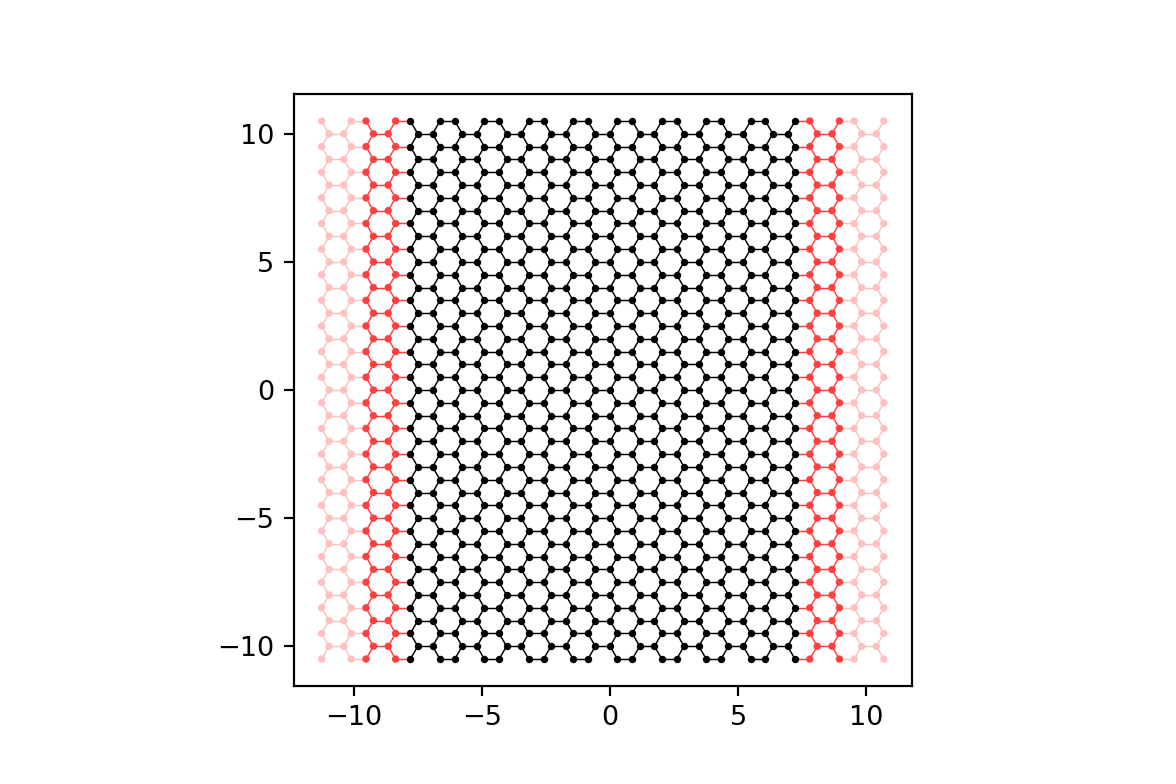
\includegraphics[width=0.45\textwidth]{./media/img1.png}
%     \caption{Some figure}
%     \label{fig:fig1}
%     \end{center}
% \end{figure}

%%%%%%%%%%%%%%
% References %
%%%%%%%%%%%%%%

\nocite{*}
\bibliographystyle{plain}
\bibliography{references}

%%%%%%%%%%%%%%
% Appendices %
%%%%%%%%%%%%%%
\appendix
\section{Some appendix}
\subsection{Some subsection}

% \begin{figure}[htb]
%     \begin{minipage}[t]{.49\textwidth}
%         \centering
%         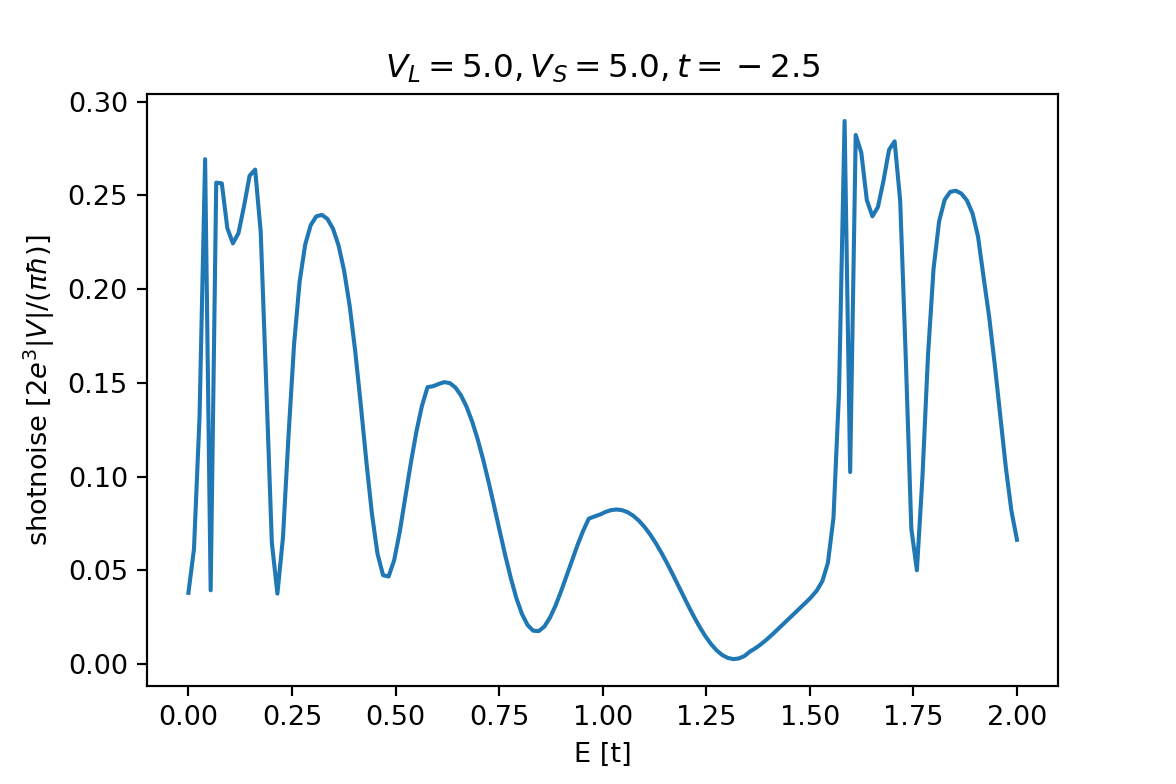
\includegraphics[width=\textwidth]{./media/img2.png}
%         \caption{Image 2}\label{fig:fig2}
%     \end{minipage}
%     \hfill
%     \begin{minipage}[t]{.49\textwidth}
%         \centering
%         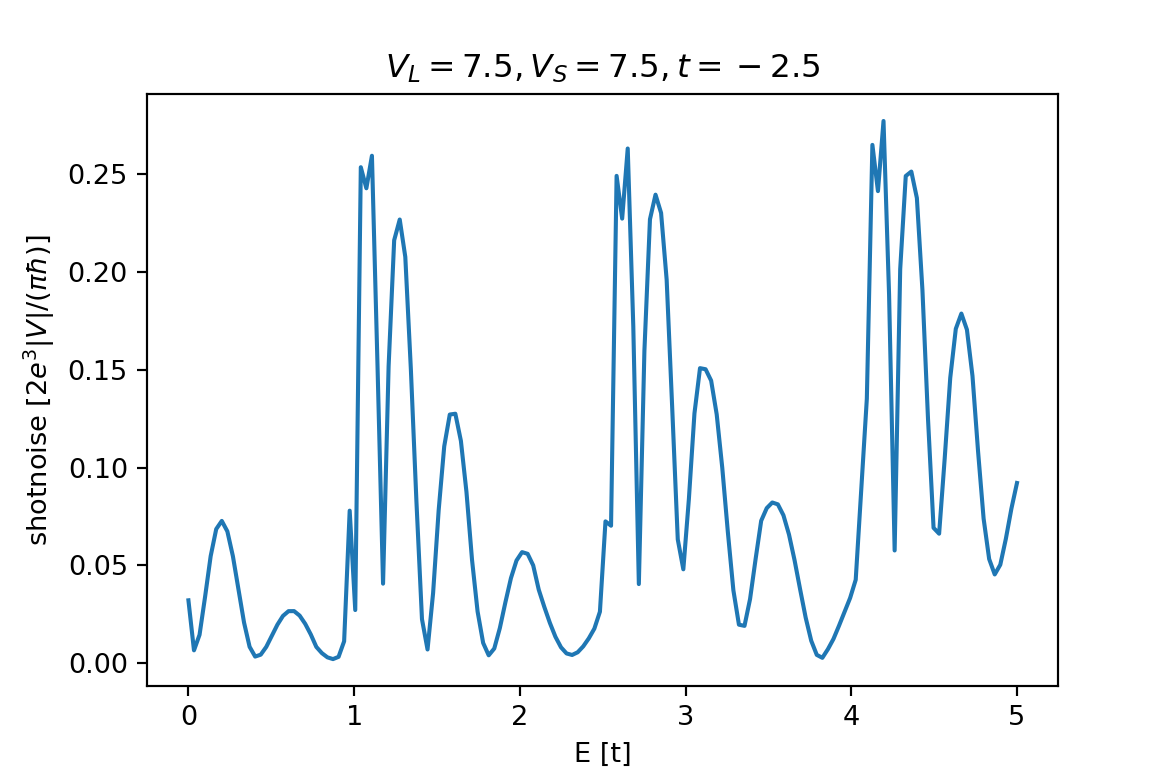
\includegraphics[width=\textwidth]{./media/img3.png}
%         \caption{Image 3}\label{fig:fig3}
%     \end{minipage}
% \end{figure}


\end{document}

